\documentclass[aspectratio=169]{beamer}

% Carrega o arquivo específico innertheme
\useinnertheme{slidestech} 
\usecolortheme[enfase=fisica]{slidestech}
\setbeamercolor{title}{fg=black, bg=gray!20}


\title{Testando Inner Theme}
\subtitle{Subtítulo de Exemplo}
\author{Seu Nome}
\institute{Sua Instituição}
\titlegraphic{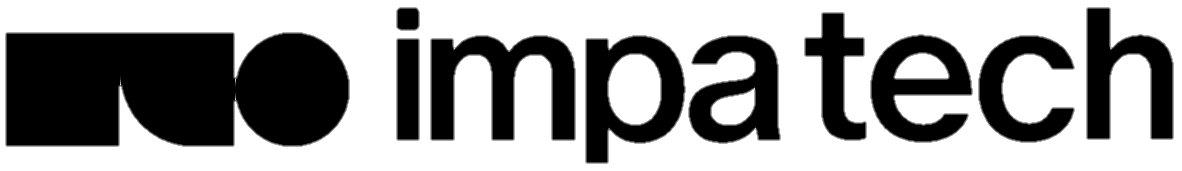
\includegraphics[width = 4.5cm]{../images/logo_03.png}}
\date{\today}

\begin{document}

\maketitle % Testa a title page já implementada

\begin{frame}{Sumário}

\tableofcontents
    
\end{frame}

\section{Listas}

\subsection{Itemize}
\begin{frame}{Itemize}
\begin{itemize}
    \item Item 1
    \begin{itemize}
        \item Item 1.1
        \begin{itemize}
            \item Item 1.1.1
        \end{itemize}
    \end{itemize}
    \item Item 2
\end{itemize}
\end{frame}

\subsection{Enumerate}
\begin{frame}{Enumerate}
\begin{enumerate}
    \item Item 1
    \begin{enumerate}
        \item Item 1.1
        \begin{enumerate}
            \item Item 1.1.1
        \end{enumerate}
    \end{enumerate}
    \item Item 2
\end{enumerate}
\end{frame}

\section{Texto}

\subsection{Texto com destaques}

\begin{frame}{Texto com destaques}
    
Este é um texto normal. \alert{Este é um texto destacado.} E este é outro texto normal.
\end{frame}

\section{Blocos}

\subsection{Teorema e Prova}

\begin{frame}{Teorema e prova}

\begin{theorem}[(Infinidade dos Primos).]
    Existem infinitos números primos.
  \end{theorem}

  \begin{proof}
    Suponha que existam apenas finitamente muitos primos $p_1, p_2, \dots, p_n$. 
    
    Considere o número $P = (p_1 \times p_2 \times \dots \times p_n) + 1$.
    
    \begin{itemize}
        \item $P$ não é divisível por nenhum dos primos da nossa lista, pois o resto da divisão por qualquer $p_i$ será sempre $1$.
        \item Logo, ou $P$ é ele próprio um novo primo, ou possui um fator primo que não está na lista original.
    \end{itemize}
    
    Em ambos os casos, encontramos um primo que não estava no conjunto finito original, gerando uma contradição. Portanto, o conjunto dos primos é infinito.
  \end{proof}
    
\end{frame}

\subsection{Exemplo e Alerta}

\begin{frame}{Exemplo}

\begin{exampleblock}{Exemplo}
    Isso é um exemplo
\end{exampleblock}
    
\end{frame}

\begin{frame}{Alerta}

\begin{alertblock}{Alerta}
    Isto é um bloco de aviso
\end{alertblock}
    
\end{frame}

\begin{frame}{Bloco padrão}

\begin{block}{Bloco}
    Este é o bloco padrão
\end{block}
    
\end{frame}

% Frame limpo, fundo branco
\begin{frame}[standout]
  Obrigada!
\end{frame}

% Fundo na cor de ênfase, texto branco
\begin{frame}[standout={bg=fisica300, fg=white}]
  Até a próxima!
\end{frame}

% COM bloco — o standoutbox vai DENTRO do frame
\begin{frame}[standout]
  \begin{standoutbox}
    It has survived not only many decades, but also the leap into electronic typesetting, remaining essentially unchanged. It was popularised thanks to these sheets and more recently with desktop publishing software including versions of Lorem Ipsum.
  \end{standoutbox}
\end{frame}

% Bloco + fundo colorido
\begin{frame}[standout={bg=pink}]
  \begin{standoutbox}
    Bloco sobre fundo pink
  \end{standoutbox}
\end{frame}

% Cor da ênfase (padrão) — verde em física, rosa em matemática, etc.
\begin{frame}[standout]
  \begin{standoutbox}
    Dentro de um bloco
  \end{standoutbox}
\end{frame}

% Cor escolhida manualmente
\begin{frame}[standout]
  \begin{standoutbox}[matematica300]
    Bloco rosa
  \end{standoutbox}
\end{frame}

\begin{frame}[standout]
  \begin{standoutbox}[computacao300]
    Bloco laranja
  \end{standoutbox}
\end{frame}

\end{document}